\subsection{Stechdorn}
\textit{(ygu)} Der Stechdorn hat die Aufgabe ein Setzloch durch Verdrängung der Topferde auszuheben und anschliessend die fallenden NemaCaps ins Setzloch zu leiten. Dafür wurde auf einen gelochten Stechdorn bewusst verzichtet, da man das Risiko von Verstopfungen nicht eingehen möchte. Mit der realisierten Konstruktion wird dieses Risiko eliminiert. 
\newline

\subsubsection{Aufbau}
Der Stechdorn besteht aus mehreren Teilen, wobei diese über eine lineare Führung (Punkt 5 in Abbildung \ref{fig:details_stechdorn}) verbunden sind. Dabei wird das Haupt (1) an der Verstellmechanik montiert und macht die Translation der Setzeinheit mit. Sobald der untere Teil (2, 3) in die Topferde einsticht, fährt die Spitze an den oberen Anschlag der Führung (Detail A). Bei der Bewegung zurück nach oben, öffnet sich die Spitze wieder und das NemaCaps kann durch den Kanal (8) ins ausgehobene Setzloch fallen (Detail B). Diese Bewegung soll nur durch die Gewichts- sowie Trägheitskraft der Spitze ausgelöst werden. Falls die Spitze zu leicht ist, um sich durch die Bewegung zu öffnen, kann in der Spitze Blei im vorgesehenen Hohlraum eingefüllt werden. Dafür ist ein Füllloch (4) vorgesehen, welches mit einer Madenschraube M6 verschlossen wird.
\newline
Folgende Überlegungen geben die Lage der linearen Führung vor:
\begin{itemize}
	\item Die lineare Führung soll möglichst parallel zur Bewegungsachse der Setzeinheit verlaufen, sodass möglichst keine Radialkräfte auf den Dorn wirken.
	
	\item Wiederum muss eine seitliche Öffnung der Spitze soweit geschehen, dass die Öffnung (9) frei über dem Setzloch steht (Detail B) und ein freier Fall des NemaCaps möglich ist.
	
	\item Der maximale Weg der Spitze in vertikaler Richtung beschränkt durch die maximale Hublänge der Spindel. Dabei ist der Abstand A in den Berechnungen (Siehe Anhang: \textit{Auslegung Spindel}) mit 15mm angenommen. Die Umsetzung überschreitet diese Annahme um 1mm, bewegt jedoch im angemessenem Rahmen.
\end{itemize}

	\begin{figure}[H]
	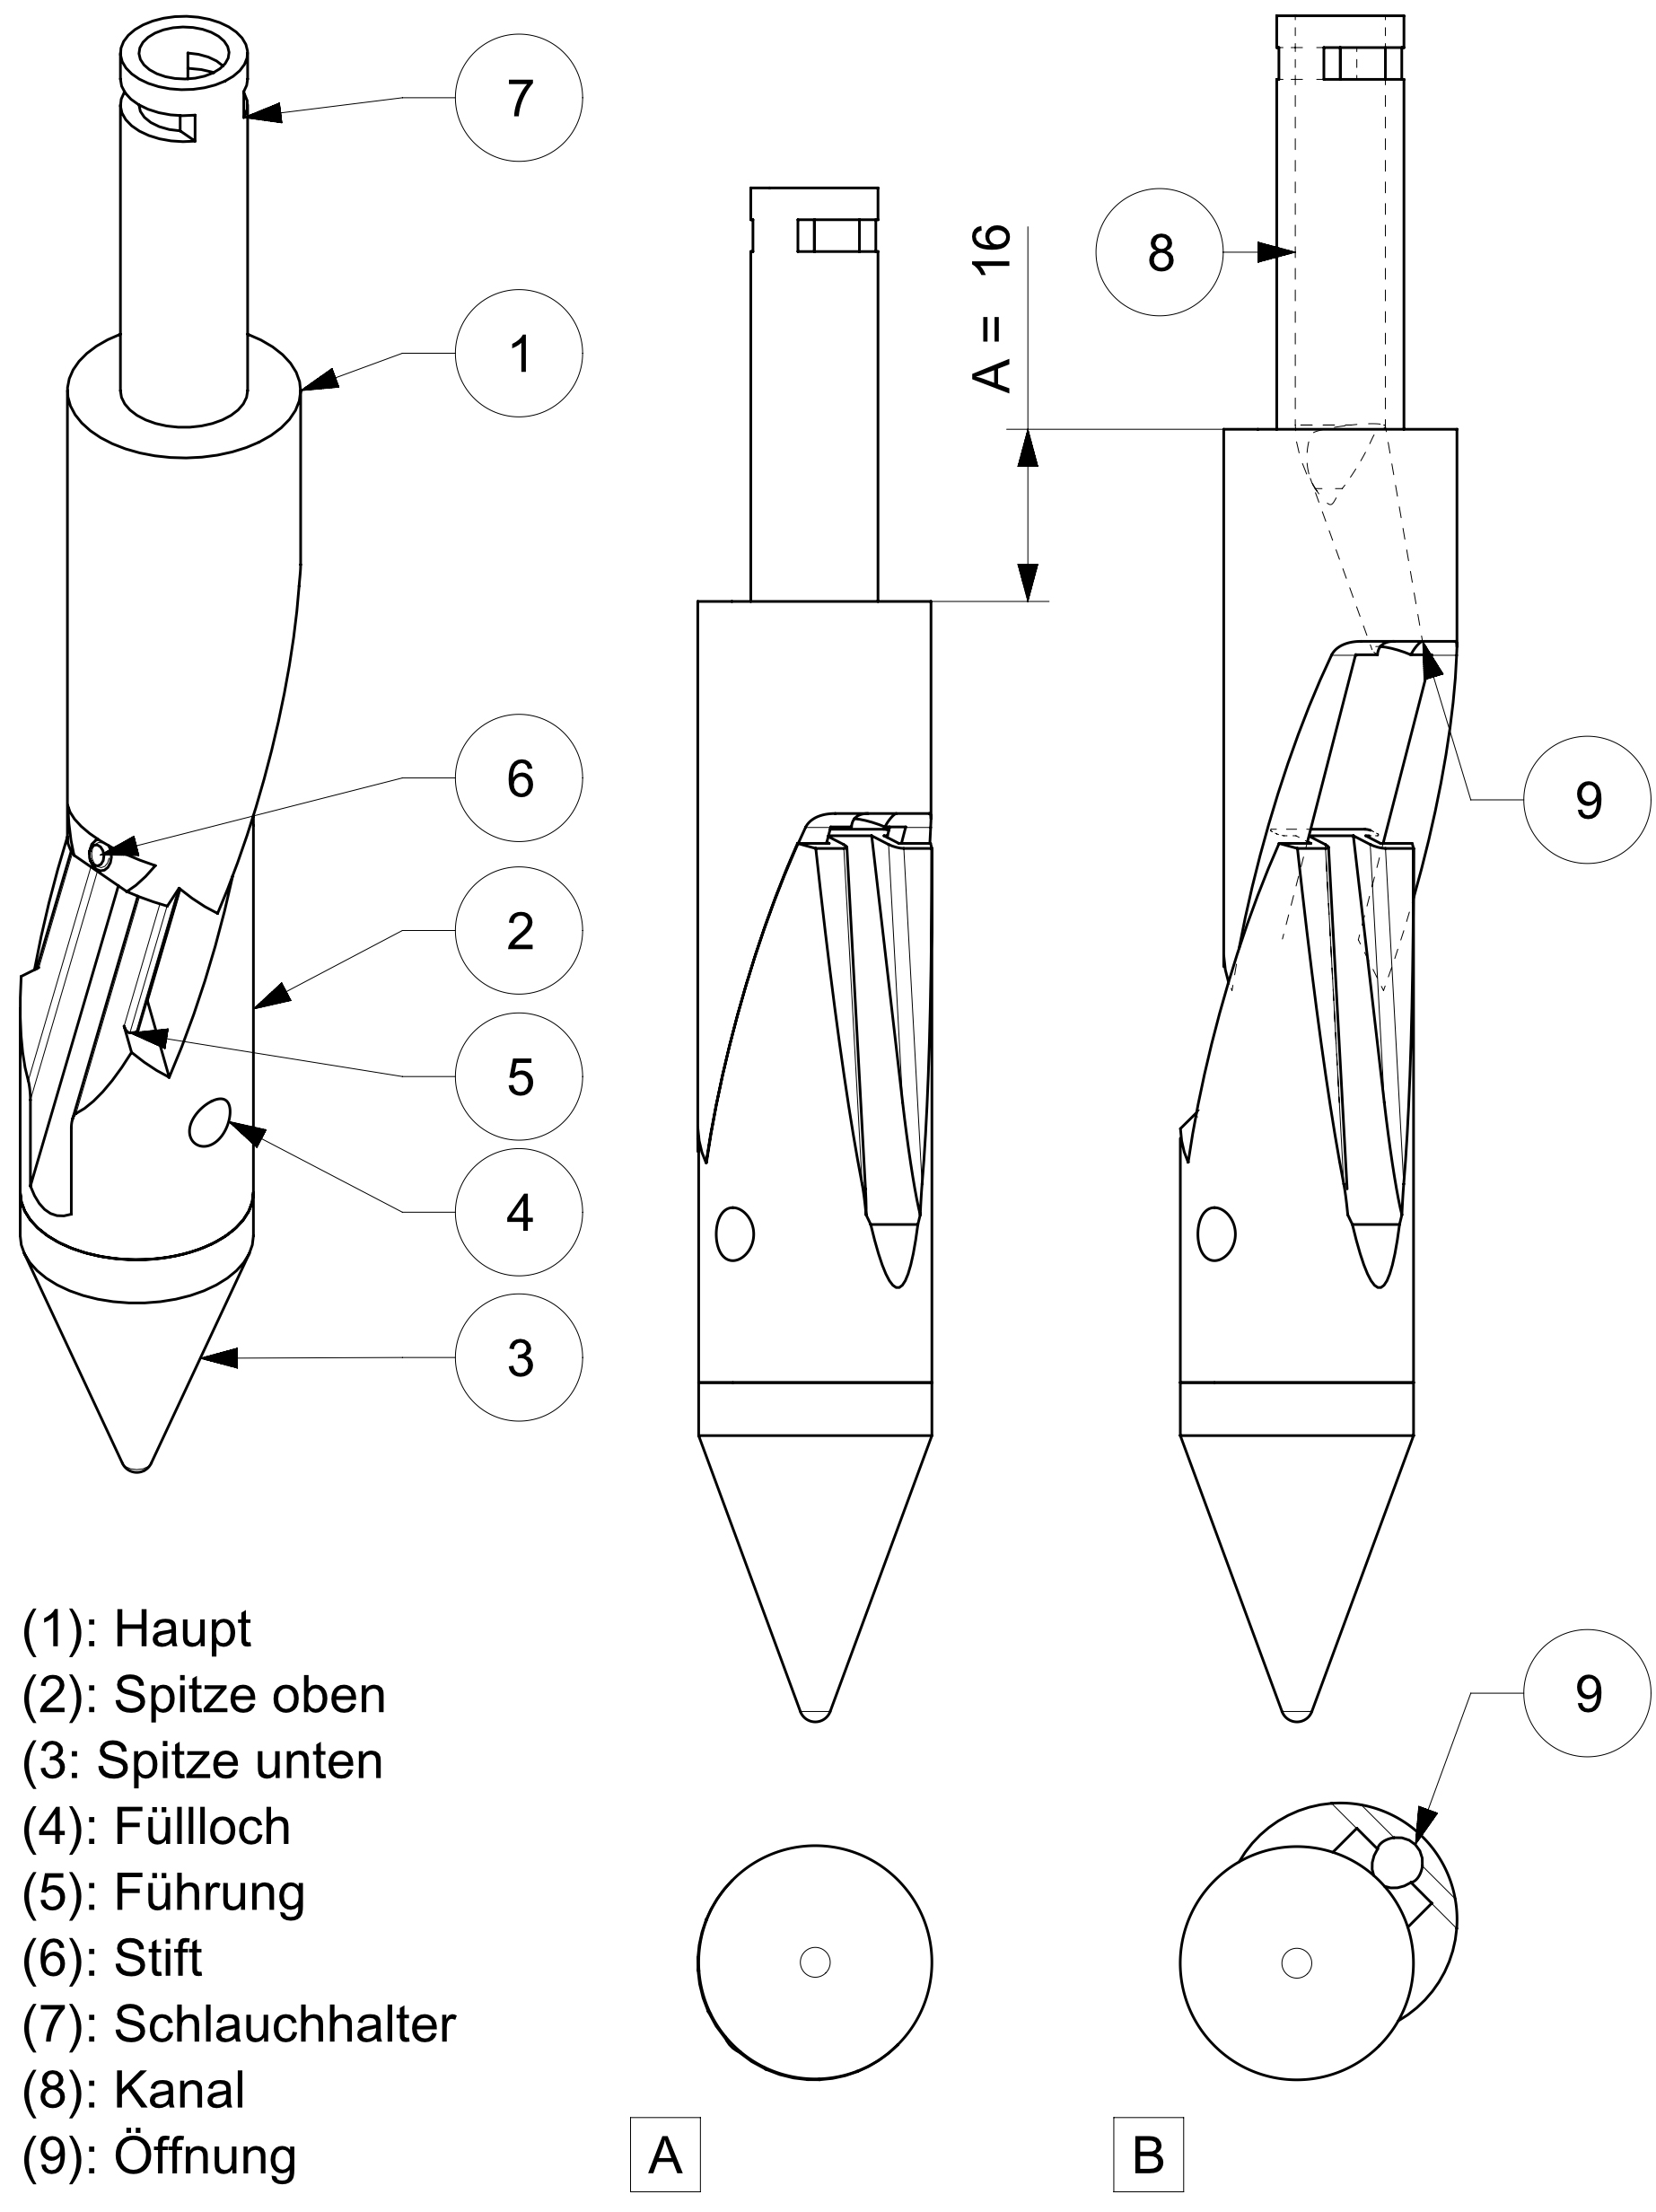
\includegraphics[scale=1.0]{Illustrationen/6-Umsetzung/details_stechdorn.jpg}
	\caption{Übersicht des Stechdorns}
	\label{fig:details_stechdorn}
	\end{figure}
\subsubsection{Haupt}
Das Haupt des Stechdorns nimmt neben der linearen Führung der Spitze noch folgende Aufgaben wahr:
\begin{itemize}
	\item Es verbindet den Schlauch mit dem Stechdorn. Dafür kann der Schlauch oben eingeführt werden und am Schlauchhalter (Punkt 12 in Abbildung \ref{fig:details_haupt}) mit einem Kabelbinder montiert werden.
	
	\item Es lenkt das fallende NemaCap mit dem Kanal (8) zur vorgesehen Öffnung und dient somit der Platzierung.
	
	\item Mit der Anbringung eines Stiftes (13) wird der untere Anschlag der Führung gewährleistet. 
		
	\item Die Montage des Dorns an der Verstellmechanik.
\end{itemize}

	\begin{figure}[H]
	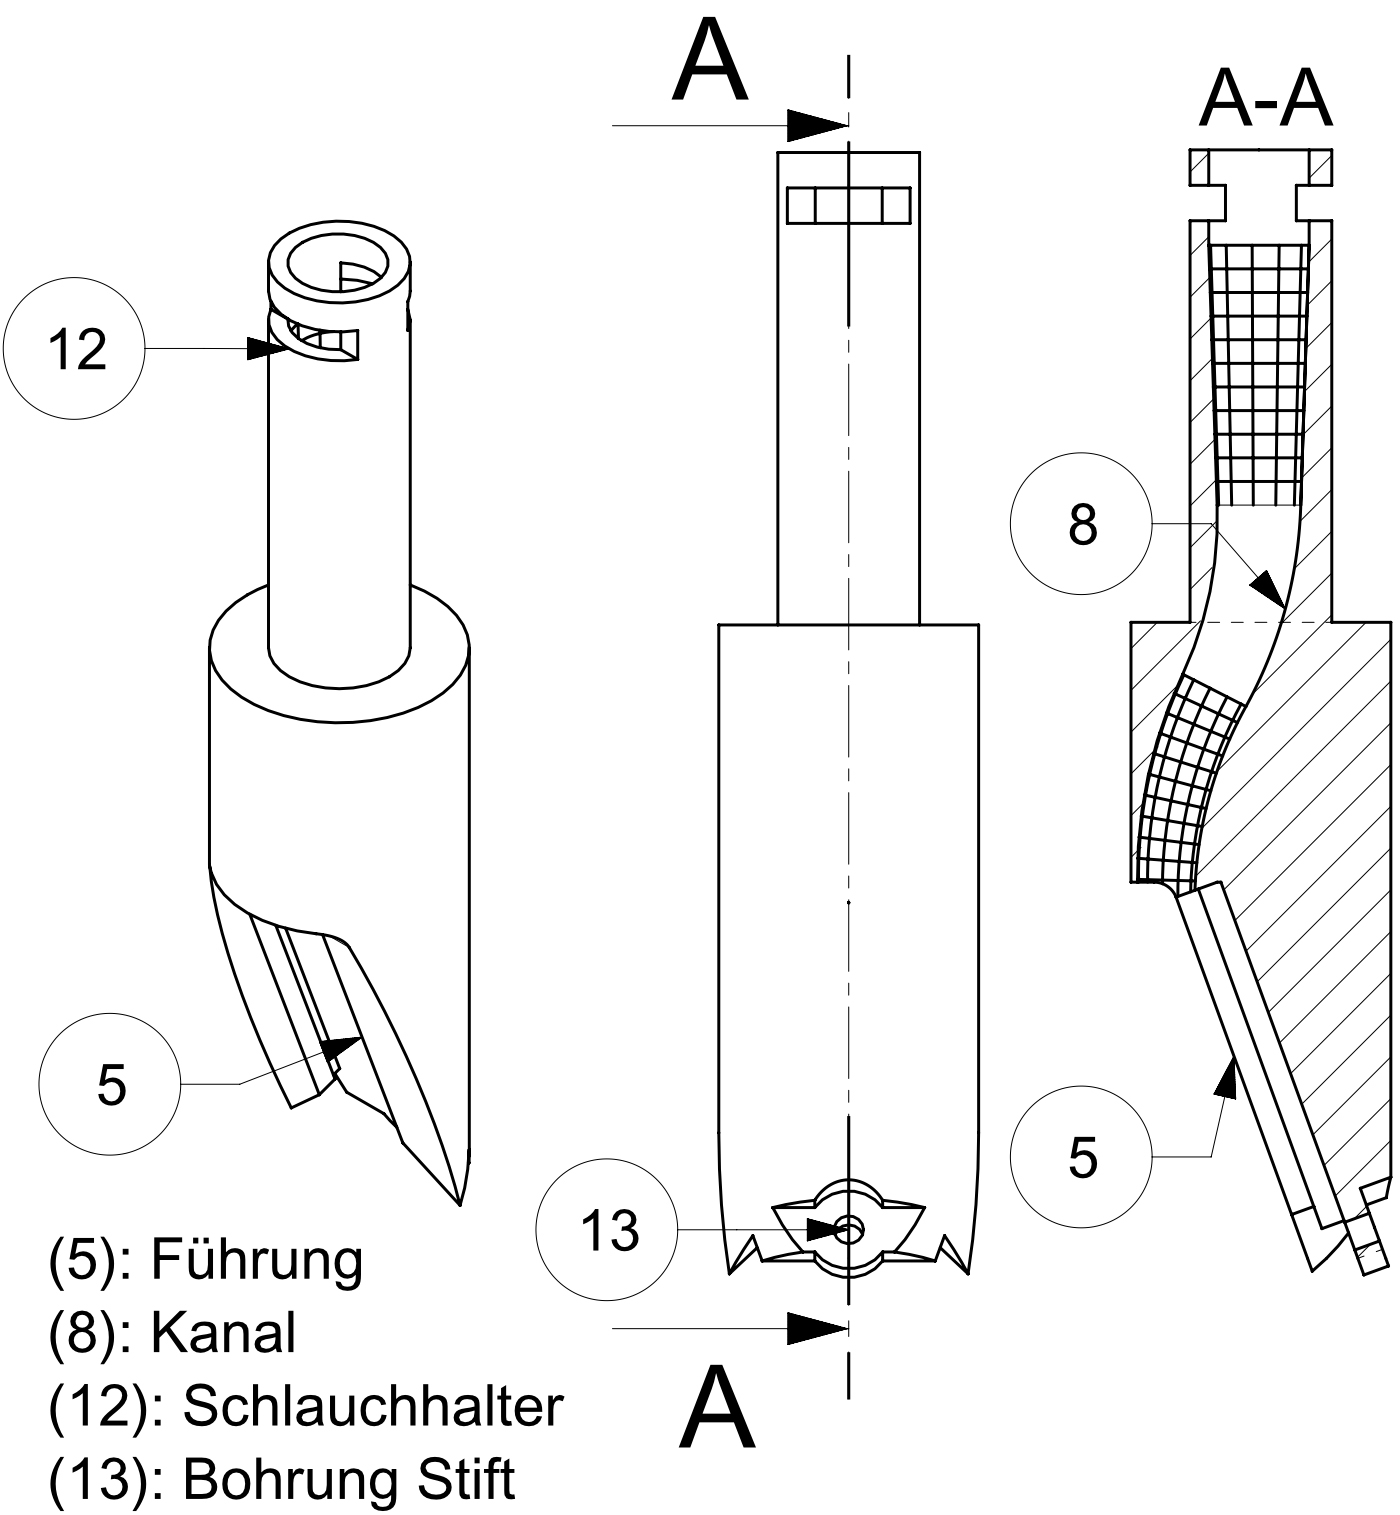
\includegraphics[scale=1.0]{Illustrationen/6-Umsetzung/details_haupt.jpg}
	\caption{Details zum Haupt}
	\label{fig:details_haupt}
	\end{figure}

\subsubsection{Spitze oben}
An der Spitze oben sind folgende konstruktive Überlegungen hervorzuheben:
\begin{itemize}
	\item Die lineare Führung ist als breites T-Profil umgesetzt (Detail A in Abbildung \ref{fig:details_spitze_oben}). Dabei ist der Steg 1.8mm dick (Mass E). Als Spielmass zwischen beiden Führungsteilen wird in alle Richtungen 0.25mm verwendet.
	
	\item Bei ausgefahrener Spitze beträgt die verbleibende Länge der Führung 11mm (Mass D). Gemäss betreuendem Dozenten (Marco De Angelis) ist das Verhältnis p von Stegdicke zu verbleibender Länge essentiel bei der Realisation von linearen Führungen dieser Art. Ideal ist ein Verhältnis von 8 ... 10 anzustreben. in diesem Fall beträgt das Verhältnis p:
	
	\begin{equation}
	p=\frac{verbleibende Fuehrung}{Stegdicke}=\frac{D}{E}=\frac{11mm}{1.8mm}=6.11
	\end{equation}
		
	Ob ein Verhältnis von 6.1 für eine funktionierende Führung ausreicht, wird die Inbetriebnahme zeigen. Allenfalls müssen diese Parameter angepasst werden.
	
	\item Da die Spitze direkt an der Topferde ausgesetzt ist, muss mit Rückständen von Erdpartikel gerechnet werden. Dabei ist die Führung ein sensitiver Teil, deren Funktion bei Kontakt mit Erdpartikeln beeinträchtigt werden kann. Um das Risiko zu mindern, wurden vorbeugende Massnahmen in der Konstruktion berücksichtigt. Ein Auslauf der Führung (11) und zwei Fasen (10) sollen die Ansammlung von Erdpartikeln verhindern.
	\end{itemize}
	\begin{figure}[H]
	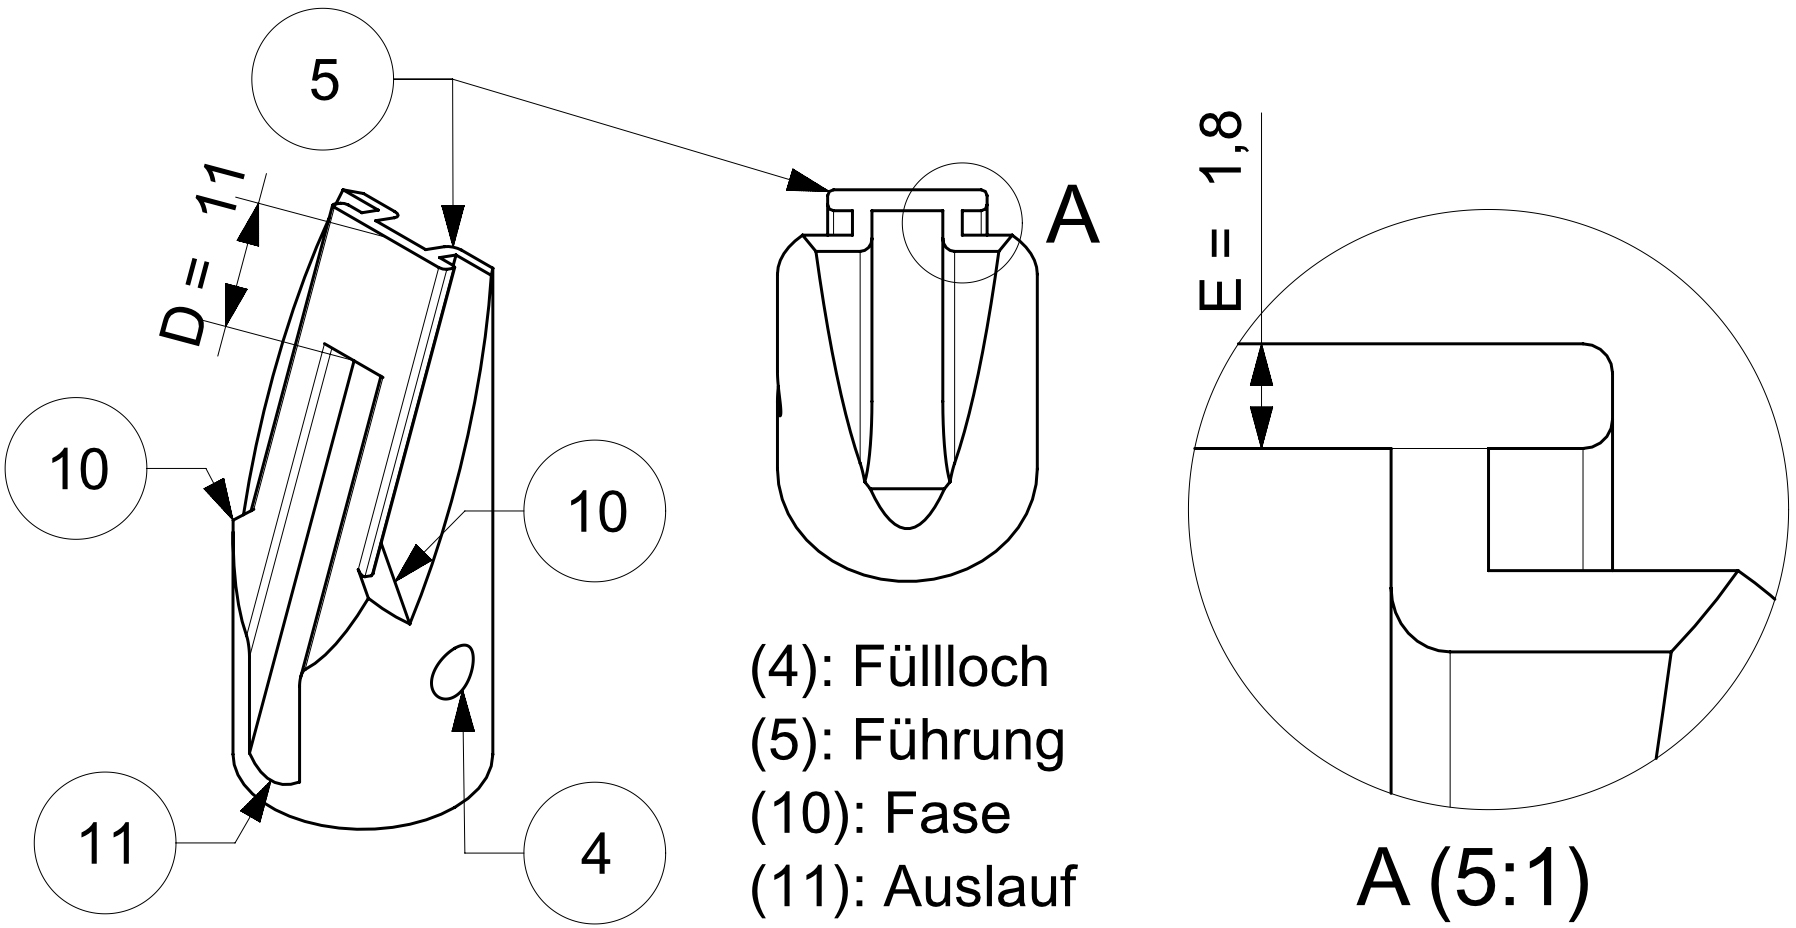
\includegraphics[scale=1.0]{Illustrationen/6-Umsetzung/details_spitze_oben.jpg}
	\caption{Details Spitze oben}
	\label{fig:details_spitze_oben}
	\end{figure}

\subsubsection{Materialwahl und Fertigungsverfahren}
Die komplexe Geometrie dieser Teile sind ausschlaggebend, dass Rapid Prototyping als Fertigungsverfahren gewählt wird. Bewusst wird die Interalbauweise für den Stechdorn genutzt, um viele Funktionen in einem Teil zu vereinen. Durch erhöhten Anforderungen an das Gewicht wird ein Kunststoff (ABS) als Material verwendet. Dabei ist es möglich, dass ein Teil mehrmals gedruckt wird, da das optimale Spielmass der linearen Führung iterativ durch zielgerichtetes Ausprobieren gefunden werden muss. 

\subsubsection{Schlauch}
Für den Transport der NemaCaps zwischen Vereinzelung und Stechdorn wird die Gravitation verwendet. Dabei werden die fallenden NemaCaps durch einen Pneumatikschlauch geleitet. Weiter stellt der Schlauch sicher, dass eine flexible Verbindung zum bewegten Stechdorn existiert. In der Pneumatik sind folgende Schlauchdimensionen gängig \cite{camozzi}:
\newline
\begin{table}[H]
\begin{tabular}{|c|c|}
	\hline 
	Aussendurchmesser D [mm] & Innendurchmesser d [mm] \\ 
	\hline 
	5 & 3 \\ 
	\hline 
	6 & 4  \\ 
	\hline 
	8 & 6 \\ 
	\hline 
	10 & 8  \\ 
	\hline 
\end{tabular}
	\caption{gängige Schlauchdimensioen}
	\label{tab:Schlauchdimensioen}
\end{table}

Für die Wahl der Schlauches stehen sich zwei widersprüchliche Aspekte gegenüber:
\begin{itemize}
	\item NemaCaps haben einen Durchmesser bis zu 3.6mm. Für einen freien Fall soll ein möglichst grosser Freiraum zur Schlauchinnenwand herrschen.
	
	\item Ein grosser Aussendurchmesser des Schlauches hat direkten Einfluss auf die Schlauchkupplungen sowie die Verstellmechanik. Dadurch werden diese Komponenten grösser. Der Lochabstand der Lochmaske steigt an und die Verstellmechanik muss grösser dimensioniert werden. Dies bedeutet mehr translatorisch beschleunigte Masse durch die Spindel. Somit ist hierfür die Wahl eines kleinen Schlauchdurchmessers vorteilhaft.
\end{itemize}
Dieser Zielkonflikt beider Aspekte bedeutet, dass die optimale Wahl des Schlauches ein Kompromiss sein muss. Daher wird ein Schlauch mit den Dimensionen 8/6 (D/d) verwendet.
\newline
Die Flexibilität wird durch das Material massgebend beeinflusst. Da keine Herstellerangaben dafür verfügbar sind, werden die Materialien Polyurethan sowie Polyamid (Nylon) für die Inbetriebnahme bestellt und dort miteinander verglichen.
